\subsection{Éléments de jeu}

\begin{figure}[h!]
        \centering
        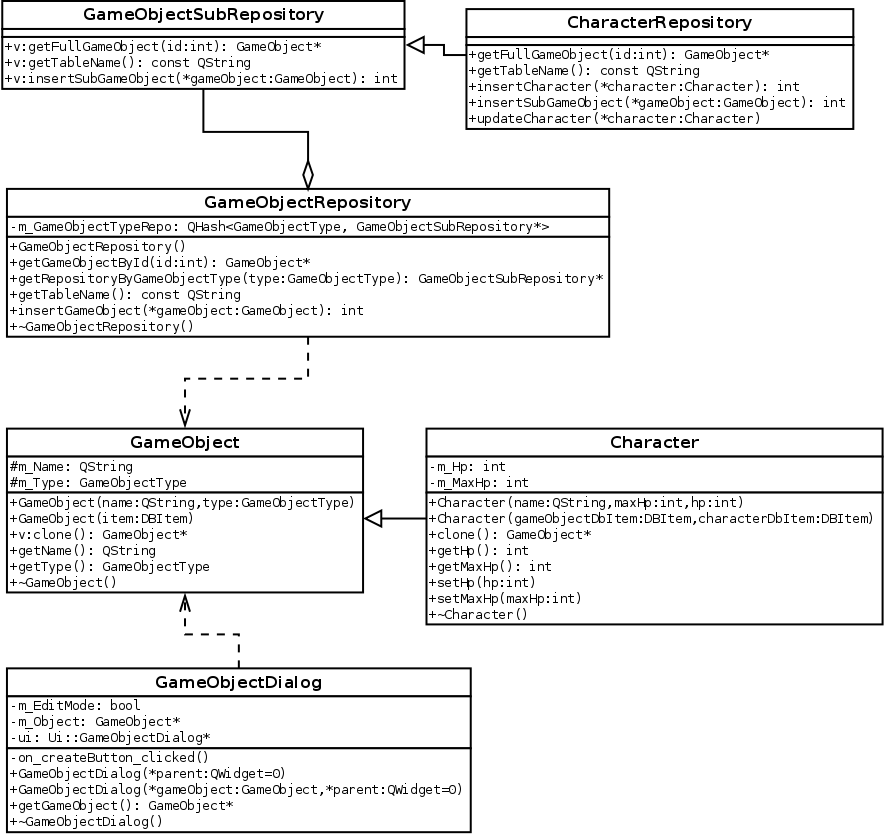
\includegraphics[width=\textwidth]{img/gameobject_uml.png}
        \caption{Diagramme UML des éléments de jeu}
\end{figure}

Un élément de jeu est représenté par la classe GameObject. Cette classe hérite de DBItem afin de pouvoir être sérialisée pour être insérée dans la base de données, et désérialisée pour pouvoir reconstruire l'objet après récupération d'informations dans la base de données. Un GameObject possède un nom ainsi qu'un type afin de savoir quel type d'objet doit être inséré/reconstruit en base de données. De plus, cette classe est liée à la table \emph{gameobject} de la bdd, et les requêtes liées à celles-ci sont stockées dans la classe GameObjectRepository.\\

Un Character est un GameObject et représente un personnage dans le jeu. Un Character ne possède que des points de vie pour le moment mais pourrait posséder d'autres éléments tels que des caractéristiques (force, agilité, ...). Cette classe est liée à la table \emph{character} de la bdd, et les requêtes liées sont stockées dans la classe CharacterRepository.\\

Les éléments de jeu sont utilisés dans les TokenItems et les Sprites. A la création d'un Sprite (lors d'un ajout sur la carte) le GameObject possédé par le TokenItem associé au Sprite est copié dans ce dernier.\\

\begin{figure}[h!]
        \centering
        \begin{subfigure}[h!]{0.7\textwidth}
                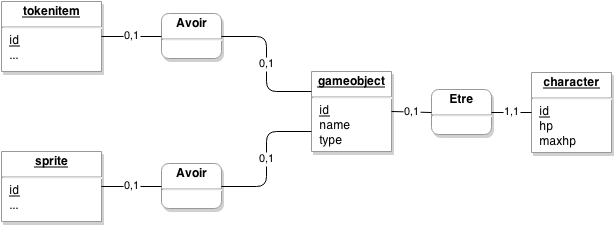
\includegraphics[width=\textwidth]{img/gameobject_MCD.png}
                \caption{Modèle Conceptuel des Données}
        \end{subfigure}

        \begin{subfigure}[h!]{0.5\textwidth}
                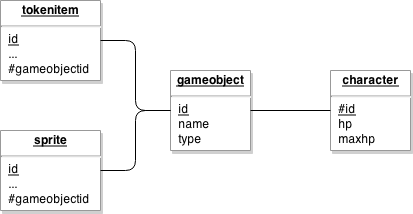
\includegraphics[width=\textwidth]{img/gameobject_MLD.png}
                \caption{Modèle Logique des Données}
        \end{subfigure}
        \caption{MCD et MLD de la base données concernant les GameObjects}
        \label{fig:GameObjectsBDD}
\end{figure}

Les Schémas ci-dessus représentent la modélisation de la base de données (MCD et MLD) concernant les GameObjects. Un élément notable est que la table character a pour clé primaire id qui fait référence à une id de la table gameobject. Ainsi, un character et son gameobject lié peuvent être facilement récupérables de la base de données à partir d'une même id.\\

Pour le moment, les seuls éléments de jeu disponibles sont les personnages. Nous pourrions cependant penser à d'autres éléments, par exemple du terrain, ou encore des objets qu'un personnage peut équiper et des consommables.\\